\documentclass[10pt]{article}
\usepackage{fullpage}
\usepackage{epsf}
\usepackage{../pplmanual}
\NeedsTeXFormat{LaTeX2e}
\typeout{^^J^^J
Parallel Programming Laboratory^^J
Manual Style^^J
Written by Milind A. Bhandarkar, 12/00^^J}

%%% Make it possible for both ps and pdf to be generated
\newif\ifpdf
\ifx\pdfoutput\undefined
  \pdffalse
\else
  \pdfoutput=1
  \pdftrue
\fi

\ifpdf
  \pdfcompresslevel=9
\fi

%%% Imported from fullpage.sty, since it is not always available
\topmargin 0pt
\advance \topmargin by -\headheight
\advance \topmargin by -\headsep

\textheight 8.9in

\oddsidemargin 0pt
\evensidemargin \oddsidemargin
\marginparwidth 1.0in

\textwidth 6.5in
%%% end import from fullpage

%%% Commonly Needed packages
\usepackage{graphicx,color,calc}
\usepackage{makeidx}
\usepackage{alltt}

%%% Commands for uniform looks of C++, Charm++, and Projections
\newcommand{\CC}{C\kern -0.0em\raise 0.5ex\hbox{\normalsize++}}
\newcommand{\emCC}{C\kern -0.0em\raise 0.4ex\hbox{\normalsize\em++}}
\newcommand{\charmpp}{\sc Charm++}
\newcommand{\projections}{\sc Projections}
\newcommand{\converse}{\sc Converse}
\newcommand{\ampi}{\sc AMPI}

%%% Commands to produce margin symbols
\newcommand{\new}{\marginpar{\fbox{\bf$\mathcal{NEW}$}}}
\newcommand{\important}{\marginpar{\fbox{\bf\Huge !}}}
\newcommand{\experimental}{\marginpar{\fbox{\bf\Huge $\beta$}}}

%%% Commands for manual elements
\newcommand{\zap}[1]{ }
\newcommand{\function}[1]{{\noindent{\textsf{#1}}\\}}
\newcommand{\cmd}[1]{{\noindent{\textsf{#1}}\\}}
\newcommand{\args}[1]{\hspace*{2em}{\texttt{#1}}\\}
\newcommand{\param}[1]{{\texttt{#1}}}
\newcommand{\kw}[1]{{\textsf{#1}}}
\newcommand{\uw}[1]{{\textsl{#1}}}
\newcommand{\desc}[1]{\indent{#1}}

%%% Commands needed for Maketitle
\newcommand{\@version}{}
\newcommand{\@credits}{}
\newcommand{\version}[1]{\renewcommand{\@version}{#1}}
\newcommand{\credits}[1]{\renewcommand{\@credits}{#1}}

%%% Print the License Page
\newcommand{\@license}{%
 \begin{center}
   {University of Illinois}\\
   {\charmpp/\converse\ Parallel Programming System Software}\\
   {Non-Exclusive, Non-Commercial Use License}\\
 \end{center}
 \rule{\textwidth}{1pt}
{\tiny
Upon execution of this Agreement by the party identified below (``Licensee''),
The Board of Trustees of the University of Illinois  (``Illinois''), on behalf
of The Parallel Programming Laboratory (``PPL'') in the Department of Computer
Science, will provide the \charmpp/\converse\ Parallel Programming System
software (``\charmpp'') in Binary Code and/or Source Code form (``Software'')
to Licensee, subject to the following terms and conditions. For purposes of
this Agreement, Binary Code is the compiled code, which is ready to run on
Licensee's computer.  Source code consists of a set of files which contain the
actual program commands that are compiled to form the Binary Code.

\begin{enumerate}
  \item
    The Software is intellectual property owned by Illinois, and all right,
title and interest, including copyright, remain with Illinois.  Illinois
grants, and Licensee hereby accepts, a restricted, non-exclusive,
non-transferable license to use the Software for academic, research and
internal business purposes only, e.g. not for commercial use (see Clause 7
below), without a fee.

  \item 
    Licensee may, at its own expense, create and freely distribute
complimentary works that interoperate with the Software, directing others to
the PPL server (\texttt{http://charm.cs.uiuc.edu}) to license and obtain the
Software itself. Licensee may, at its own expense, modify the Software to make
derivative works.  Except as explicitly provided below, this License shall
apply to any derivative work as it does to the original Software distributed by
Illinois.  Any derivative work should be clearly marked and renamed to notify
users that it is a modified version and not the original Software distributed
by Illinois.  Licensee agrees to reproduce the copyright notice and other
proprietary markings on any derivative work and to include in the documentation
of such work the acknowledgement:

\begin{quote}
``This software includes code developed by the Parallel Programming Laboratory
in the Department of Computer Science at the University of Illinois at
Urbana-Champaign.''
\end{quote}

Licensee may redistribute without restriction works with up to 1/2 of their
non-comment source code derived from at most 1/10 of the non-comment source
code developed by Illinois and contained in the Software, provided that the
above directions for notice and acknowledgement are observed.  Any other
distribution of the Software or any derivative work requires a separate license
with Illinois.  Licensee may contact Illinois (\texttt{kale@cs.uiuc.edu}) to
negotiate an appropriate license for such distribution.

  \item
    Except as expressly set forth in this Agreement, THIS SOFTWARE IS PROVIDED
``AS IS'' AND ILLINOIS MAKES NO REPRESENTATIONS AND EXTENDS NO WARRANTIES OF
ANY KIND, EITHER EXPRESS OR IMPLIED, INCLUDING BUT NOT LIMITED TO WARRANTIES OR
MERCHANTABILITY OR FITNESS FOR A PARTICULAR PURPOSE, OR THAT THE USE OF THE
SOFTWARE WILL NOT INFRINGE ANY PATENT, TRADEMARK, OR OTHER RIGHTS.  LICENSEE
ASSUMES THE ENTIRE RISK AS TO THE RESULTS AND PERFORMANCE OF THE SOFTWARE
AND/OR ASSOCIATED MATERIALS.  LICENSEE AGREES THAT UNIVERSITY SHALL NOT BE HELD
LIABLE FOR ANY DIRECT, INDIRECT, CONSEQUENTIAL, OR INCIDENTAL DAMAGES WITH
RESPECT TO ANY CLAIM BY LICENSEE OR ANY THIRD PARTY ON ACCOUNT OF OR ARISING
FROM THIS AGREEMENT OR USE OF THE SOFTWARE AND/OR ASSOCIATED MATERIALS.

  \item 
    Licensee understands the Software is proprietary to Illinois. Licensee
agrees to take all reasonable steps to insure that the Software is  protected
and secured from unauthorized disclosure, use, or release and  will treat it
with at least the same level of care as Licensee would use to  protect and
secure its own proprietary computer programs and/or information, but using no
less than a reasonable standard of care.  Licensee agrees to provide the
Software only to any other person or entity who has registered with Illinois.
If licensee is not registering as an individual but as an institution or
corporation each member of the institution or corporation who has access to or
uses Software must agree to and abide by the terms of this license. If Licensee
becomes aware of any unauthorized licensing, copying or use of the Software,
Licensee shall promptly notify Illinois in writing. Licensee expressly agrees
to use the Software only in the manner and for the specific uses authorized in
this Agreement.

  \item
    By using or copying this Software, Licensee agrees to abide by the
copyright law and all other applicable laws of the U.S. including, but not
limited to, export control laws and the terms of this license. Illinois  shall
have the right to terminate this license immediately by written  notice upon
Licensee's breach of, or non-compliance with, any terms of the license.
Licensee may be held legally responsible for any  copyright infringement that
is caused or encouraged by its failure to  abide by the terms of this license.
Upon termination, Licensee agrees to  destroy all copies of the Software in its
possession and to verify such  destruction in writing.

  \item
  The user agrees that any reports or published results obtained with  the
Software will acknowledge its use by the appropriate citation as  follows:

\begin{quote}
``\charmpp/\converse\ was developed by the Parallel Programming Laboratory in
the Department of Computer Science at the University of  Illinois at
Urbana-Champaign.''
\end{quote}

Any published work which utilizes \charmpp\ shall include the following
reference:

\begin{quote}
``L. V. Kale and S. Krishnan. \charmpp: Parallel Programming with Message-Driven
Objects. In 'Parallel Programming using \CC' (Eds. Gregory V. Wilson and Paul
Lu), pp 175-213, MIT Press, 1996.''
\end{quote}

Any published work which utilizes \converse\ shall include the following
reference:

\begin{quote}
``L. V. Kale, Milind Bhandarkar, Narain Jagathesan, Sanjeev Krishnan and Joshua
Yelon. \converse: An Interoperable Framework for Parallel Programming.
Proceedings of the 10th International Parallel Processing Symposium, pp
212-217, April 1996.''
\end{quote}

Electronic documents will include a direct link to the official \charmpp\ page
at \texttt{http://charm.cs.uiuc.edu/}

  \item
    Commercial use of the Software, or derivative works based thereon,
REQUIRES A COMMERCIAL LICENSE.  Should Licensee wish to make commercial use of
the Software, Licensee will contact Illinois (kale@cs.uiuc.edu) to negotiate an
appropriate license for such use. Commercial use includes: 

    \begin{enumerate}
      \item
	integration of all or part of the Software into a product for sale,
lease or license by or on behalf of Licensee to third parties, or 

      \item
	distribution of the Software to third parties that need it to
commercialize product sold or licensed by or on behalf of Licensee.
    \end{enumerate}

  \item
    Government Rights. Because substantial governmental funds have been  used
in the development of \charmpp/\converse, any possession, use or sublicense of
the Software by or to the United States government shall be subject to such
required restrictions.

  \item
    \charmpp/\converse\ is being distributed as a research and teaching tool
and as such, PPL encourages contributions from users of the code that might, at
Illinois' sole discretion, be used or incorporated to make the basic  operating
framework of the Software a more stable, flexible, and/or useful  product.
Licensees who contribute their code to become an internal  portion of the
Software agree that such code may be distributed by  Illinois under the terms
of this License and may be required to sign an  ``Agreement Regarding
Contributory Code for \charmpp/\converse\ Software'' before Illinois  can
accept it (contact \texttt{kale@cs.uiuc.edu} for a copy).
\end{enumerate}

UNDERSTOOD AND AGREED.

Contact Information:

The best contact path for licensing issues is by e-mail to
\texttt{kale@cs.uiuc.edu} or send correspondence to:

\begin{quote}
Prof. L. V. Kale\\
Dept. of Computer Science\\
University of Illinois\\
1304 W. Springfield Ave\\
Urbana, Illinois 61801 USA\\
FAX: (217) 333-3501
\end{quote}
}%tiny
 \newpage
}% end of license

\renewcommand{\maketitle}{\begin{titlepage}%
 \begin{flushright}
   {\Large
     Parallel Programming Laboratory\\
     University of Illinois at Urbana-Champaign\\
   }
 \end{flushright}
 \rule{\textwidth}{3pt}
 \vspace{\fill}
 \begin{flushright}
   \textsf{\Huge \@title \\}
 \end{flushright}
 \vspace{\fill}
 \@credits \\
 \rule{\textwidth}{3pt}
 \begin{flushright}
   {\large Version \@version}
 \end{flushright}
 \end{titlepage}
 \@license

 \tableofcontents
 \newpage
}% maketitle



\newcommand{\pose}{{\sc Pose}}

\begin{document}

%\maketitle
\begin{titlepage}
 \begin{flushright}
   {\Large
     Parallel Programming Laboratory\\
     University of Illinois at Urbana-Champaign\\
   }
 \end{flushright}
 \rule{\textwidth}{3pt}
 \vspace{\fill}
 \begin{flushright}
   \textsf{\Huge \pose{} Reference Manual \\}
 \end{flushright}
 \vspace{\fill}
 {\small \pose{} software and this manual are entirely the fault of Terry
L. Wilmarth.  Credit for Charm++ is due to the developers, past and
present, at the Parallel Programming Laboratory ({\tt
http://charm.cs.uiuc.edu}).  Questions or comments on \pose{} or this
manual can be directed to Terry at {\tt wilmarth@cse.uiuc.edu}.
} \\
 \rule{\textwidth}{3pt}
\end{titlepage}

\tableofcontents
\newpage

\section{About this manual}

This manual is {\bf UNDER CONSTRUCTION}.  It is definitely incomplete,
and probably inaccurate in some cases.  Please e-mail Terry, {\tt
  wilmarth@uiuc.edu} if you find any problems with the manual.  Thanks.

\section{About \pose{}}

\pose{} (Parallel Object-oriented Simulation Environment) is a tool for
parallel discrete event simulation (PDES) based on Charm++.  You should have
a background in object-oriented programming (preferably C++), know the
basic principles behind discrete event simulation, and be familiar
with simple parallel programming in Charm++.  

\pose{} uses the approach of message-driven execution of Charm++, but
adds the element of discrete timestamps to control when, in simulated
time, a message is executed.

Users may choose synchronization strategies (conservative or several
optimistic variants) on a per class basis, depending on the desired
behavior of the object.  However, \pose{} is intended to perform best
with a special type of {\it adaptive} synchronization strategy which
changes it's be havior on a per object basis.  Thus, other
synchronization strategies may not be properly maintained.  There are
two versions of the adaptive strategy, {\sl adapt}, a simple, stable
version, and {\sl adapt2}, the development version.

\section{Developing a model in \pose{}}

Modelling a system in \pose{} is similar to how you would model in C++ or
any OOP language.  Objects are entities that hold data, and have a
fixed set of operations that can be performed on them (methods).

Charm++ provides the parallelism we desire, but the model does not
differ dramatically from C++.  The primary difference is that objects
may exist on a set of processors, and so invoking methods on them
requires communication via messages. 

\pose{} adds to Charm++ by putting timestamps on method invocations
(events), and executing events in timestamp order to preserve the
validity of the global state.

Developing a model in \pose{} involves identifying the entities we
wish to model, determining their interactions with other entities and
determining how they change over time.

\subsection{PDES in \pose{}}

A simulation in \pose{} consists of a set of entities performing
timestamped events in parallel.  These entities are called {\sl
posers}.  \pose{} is designed to work with many such entities per
processor. The more a system can be broken down into its parallel
components when designing the simulation model, the more potential
parallelism in the final application.

A poser class is defined with a synchronization strategy associated
with it.  We encourage the use of the adaptive strategies, as
mentioned earlier.  Adaptive strategies are optimistic, and will
potentially execute events out of order, but have rollback and
cancellation messages as well as checkpointing abilities to deal with
this behind the scenes.

Execution is driven by events.  An event arrives for a poser and is
sorted into a queue by timestamp.  The poser has a local time called
object virtual time (OVT) which represents its progress through the
simulation.  When an event arrives with a timestamp $t>$OVT, the OVT is
advanced to $t$.  If the event has timestamp $t<$OVT, it maybe that
other events with greater timestamps were executed.  If this is the
case, a rollback will occur.  If not, the event is simply executed
along with the others in the queue.

Time can also pass on a poser within the course of executing an
event.  An {\sl elapse} function is used to advance the OVT.  

Currently, \pose{} has no way to specify event dependencies, so if
they exist, the programmer must handle errors in ordering carefully.
\pose{} provides a delayed error message print and abort function that
is only performed if there is no chance of rolling back the dependency
error. 

\pose{} maintains a global clock, the global virtual time (GVT), that
represents the progress of the entire simulation.  

\section{Programmer's Reference}

This section details syntax and usage of \pose{} constructs.  The last
subsection lists all constructs and their usage in brief.

\subsection{\pose{} Modules}

A \pose{} module is similar to a Charm++ module.  It is comprised of
{\tt .ci}, {\tt .h}, and {\tt .C} files.  Several posers can be
described in one module, and the module can include regular chares as
well.  The module is translated into Charm++ before the simulation can
be compiled.  This translation is performed by a Perl script called
{\sl etrans.pl} which is included with \pose{}.  It generates files
suffixed {\tt \_sim.ci}, {\tt \_sim.h}, and {\tt \_sim.C}.  

\subsection{Event Message and Poser Interface Description}

Messages, be they event messages or otherwise, are described in the
{\tt .ci} file exactly the way they are in Charm++, with the exception
that parameter marshalling cannot currently be used, and thus you must declare
them in the {\tt .h} file.  

~\\
\noindent{\tt {\bf message} {\it myMessage};}\\

Posers are described similar to chares, with a few exceptions.  First,
the {\tt poser} keyword is used to denote that the class is a \pose{}
simulation object class.  Second, event methods are tagged with the
keyword {\tt event} in square brackets. Finally, three components are
specified which indicate how objects of the poser class are to be
simulated.  The {\it sim} component controls the wrapper class and
event queue used by the object (see section ? for more on the internal
representation of a poser).  The {\it strat} component controls the
synchronization strategy the object should use ({\it i.e. optimistic}
or {\it conservative}).  The {\it rep} component specifies the global
state representation, which controls how the global state is kept
accurate depending on the synchronization strategy being used ({\it
i.e. checkpointing}).

~\\
\noindent{\tt {\bf poser} {\it mySim} : {\it sim strat rep} \{\\
\indent {\bf entry} {\it mySim}({\it myMessage} *);\\
\indent {\bf entry} [{\bf event}] void {\it myEventMethod}({\bf eventMsg} *);\\
\indent ...\\
\noindent \};}\\

Note that the constructors and event methods of a poser must take an
event message as parameter.  If there is no data (and thereby no
message defined) that needs to be passed to the method, then the
parameter should be of type {\tt eventMsg *}.  This ensures that
\pose{} will be able to timestamp the event.

\subsection{Declaring Event Messages and Posers}

Currently, event messages are declared with no reference to what they
might inherit from (unlike in Charm++).  The translator takes care of
this. In addition, they must define {\tt operator=}.

~\\
\noindent{\tt class {\it myMessage} \{\\
\indent  public:\\
\indent   int someData;\\
\indent   {\it myMessage}\& operator=(const {\it myMessage}\& obj) \{\\
\indent\indent     {\bf eventMsg}::operator=(obj);\\
\indent\indent     someData = obj.someData;\\
\indent\indent     return *this;\\
\indent   \}\\
\noindent \};}\\

Similarly, posers do not refer to a base class when they are
declared.  Posers are required to have a void constructor declared
that simply initializes the data to sensible values.  A destructor
must be provided as well.  In addition, a {\tt pup} and {\tt
operator=} must be provided.  The {\tt pup} method should call the
{\tt pup} method of the global state representation class being used.

~\\
\noindent{\tt class {\it mySim} \{\\
\indent int anInt; float aFloat; char aString[20];\\
~public:\\
\indent {\it mySim}();\\
\indent {\it mySim}({\it myMessage} *m);\\
\indent \verb|~|{\it mySim}();\\
\indent void pup(PUP::er \&p);\\
\indent {\it mySim}\& operator=(const {\it mySim}\& obj);\\
\indent void {\it myEventMethod}({\bf eventMsg} *m);\\
\indent void {\it myEventMethod}{\bf \_anti}({\bf eventMsg} *m);\\
\indent void {\it myEventMethod}{\bf \_commit}({\bf eventMsg} *m);\\
\indent ...\\
\noindent \};}\\

Further, for each event method, a commit method should be declared,
and if the synchronization strategy being used is optimistic or
involves any sort of rollback, an anti-method should also be provided.
The syntax of these declarations is shown above.  Their usage and
implementation will be described next.

\subsection{Implementing Posers}

The void constructor for a poser should be defined however the user
sees fit.  It could be given an empty body and should still work for
\pose{}.  Poser entry constructors (those described in the {\tt .ci}
file) should follow the template below:

~\\
\noindent{\tt {\it mySim}::{\it mySim}({\it myMessage} *m)\\
\noindent\{\\
\indent // initializations from $m$\\
\indent ...\\
\indent delete m;\\
\indent ...\\
\noindent \};}\\

Note that while the incoming message $m$ may be deleted here in the
constructor, event messages received on event methods should {\bf not} be
deleted.  The PDES fossil collection will take care of those.

An event method should have the following form:

~\\
\noindent{\tt void {\it mySim}::{\it myEventMethod}(eventMsg *m) \{\\
\indent // body of method \\
\noindent \};}\\

Again, $m$ is never deleted in the body of the event.  A side effect
of optimistic synchronization and rollback is that we would like the
effects of event execution to be dependent only upon the state
encapsulated in the corresponding poser.  Thus, accessing arbitrary
states outside of the simulation, such as by calling {\tt rand}, is
forbidden.  We are planning to fix this problem by adding a {\tt
  POSE\_rand()} operation which will generate a random number the first
time the event is executed, and will checkpoint the number for use in
subsequent re-executions should a rollback occur.

\subsection{Creation of Poser Objects}

Posers are created within a module using the following syntax:

~\\
\noindent {\tt int hdl = 13;  // handle should be unique\\
\noindent {\it myMessage} *m = new {\it myMessage};\\
\noindent m->someData = 34;\\
\noindent {\bf POSE\_create}({\it mySim}(m), hdl, 0);}\\

This creates a {\tt mySim} object that comes into existence at
simulation time zero, and can be referred to by the handle 13.  

Creating a poser from outside the module ({\it i.e.} from {\tt main})
is somewhat more complex:

~\\
\noindent {\tt int hdl = 13;\\
\noindent {\it myMessage} *m = new {\it myMessage};\\
\noindent m->someData = 34;\\
\noindent m->{\bf Timestamp}(0);\\
\noindent (*(CProxy\_{\it mySim} *) \& {\bf POSE\_Objects})[hdl].insert(m);}\\

This is similar to what the module code ultimately gets translated to
and should be replaced by a macro with similar syntax soon.

\subsection{Event Method Invocations}

Event method invocations vary significantly from entry method
invocations in Charm++, and various forms should be used depending on
where the event method is being invoked.  In addition, event messages
sent to an event method should be allocated specifically for an event
invocation, and cannot be recycled or deleted.

There are three ways to send events within a \pose{} module.  The first
and most commonly used way involves specifying and offset in
simulation time from the current time.  The syntax follows:

~\\
\noindent {\tt aMsg = new {\bf eventMsg};\\
\noindent {\bf POSE\_invoke}({\it myEventMethod}(aMsg), {\it
mySim}, hdl, 0);}\\

Here, we've created an {\tt eventMsg} and sent it to {\tt
myEventMethod}, an event entry point on {\tt mySim}.  {\tt mySim} was
created at handle {\tt hdl}, and we want the event to take place now,
i.e. at the current simulation time, so the offset is zero.  

The second way to send an event is reserved for use by non-poser
objects within the module.  It should not be used by posers.  This
version allows you to specify an absolute simulation time at which the
event happens (as opposed to an offset to the current time).  Since
non-poser objects are not a part of the simulation, they do not have a
current time, or OVT, by which to specify an offset.  The syntax is
nearly identical to that above, only the last parameter is an absolute
time.

~\\
\noindent {\tt aMsg = new {\bf eventMsg};\\
\noindent {\bf POSE\_invoke\_at}({\it myEventMethod}(aMsg), {\it
mySim}, hdl, 56);}\\

Posers should not use this approach because of the risk of specifying
an absolute time that is earlier than the current time on the object
sending the event.  

Using this method, event methods can be injected into the system from
outside any module, but this is not recommended.

The third approach is useful when an object send events to itself.  It
is simply a slightly shorter syntax for the same thing as {\tt
POSE\_invoke}: 

~\\
\noindent {\tt aMsg = new {\bf eventMsg};\\
\noindent {\bf POSE\_local\_invoke}({\it myEventMethod}(aMsg), offset);}\\

\subsection{Elapsing Simulation Time}

We've seen in the previous section how it is possible to advance
simulation time by generating events with non-zero offsets of current
time.  When such events are received on an object, if the object is
behind, it advances its local simulation time (object virtual time or
OVT) to the timestamp of the event.

It is also possible to elapse time on an object while the object is
executing an event.  This is accomplished thus:

~\\
\noindent {\tt {\bf elapse}(42);}\\

The example above would simulate the passage of forty-two time units
by adding as much to the object's current OVT.

\subsection{Interacting with a \pose{} Module and the \pose{} System}

\pose{} modules consist of {\tt <$modname$>.ci}, {\tt <$modname$>.h}
and {\tt <$modname$>.C} files that are translated via {\tt etrans.pl}
into {\tt <$modname$>\_sim.ci}, {\tt <$modname$>\_sim.h} and {\tt
<$modname$>\_sim.C} files.  To interface these with a main program
module, say $Pgm$ in files {\tt pgm.ci}, {\tt pgm.h} and {\tt pgm.C},
the {\tt pgm.ci} file must declare the \pose{} module as extern in the
{\tt mainmodule Pgm} block. For example:

~\\
\noindent{\tt mainmodule Pgm \{\\
\indent  extern module <$modname$>;\\
\indent  readonly CkChareID mainhandle;\\
   \\
\indent  mainchare main \{\\
\indent\indent    entry main();\\
\indent  \};\\
\noindent \};}\\

The {\tt pgm.C} file should include {\tt pose.h} and {\tt<$modname$>\_sim.h}
along with its own headers, declarations and whatever else it needs.

Somewhere in the {\tt main} function, {\tt POSE\_init()} should be
called.  This initializes all of \pose{}'s internal data structures.
Then, a termination method should be specified.  \pose{} programs can
be terminated in two ways: with inactivity detection or with an end
time.  Inactivity detection terminates after a few iterations of the
GVT determine that no events are being executed and virtual time is
not advancing.  When an end time is specified, and the GVT passes it,
the simulation exits.  Both approaches can be used separately or in
combination:

~\\
\noindent{\tt POSE\_useID();\\
\noindent POSE\_useET($t$);}\\

Now \pose{} is ready for posers.  All posers can be created at this
point, each with a unique handle.  The programmer is responsible for
choosing and keeping track of the handles created for posers.  Once
all posers are created, the simulation can be started:

~\\
\noindent{\tt POSE\_start();}\\

\subsection{Glossary of \pose{}-specific Terms}

\begin{itemize}
\item {\tt void {\bf POSE\_init}()}\\
	$\circ$ Initializes various items in \pose{}; creates the load balancer
	if load balancing is turned on; initializes the statistics
	gathering facility if statistics are turned on.\\
	$\circ$ Must be called in user's main program prior to creation of any
	simulation objects or reference to any other \pose{} construct.
\item {\tt void {\bf POSE\_start}()}\\
	$\circ$ Sets busy wait to default if none specified; starts
	quiescence detection; starts simulation timer.\\
	$\circ$ Must be called in user's main program when simulation
	should start.
\item {\tt void {\bf POSE\_registerCallBack}(CkCallback cb)}\\
	$\circ$ Registers callback function with \pose{} -- when program
	ends or quiesces, function is called.\\
	$\circ$ CkCallback is created with the index of the callback
	function and a proxy to the object that function is to be
	called on.  For example, to register the function {\tt wrapUp}
	in the main module as a callback:

\begin{verbatim}
  CProxy_main M(mainhandle);
  POSE_registerCallBack(CkCallback(CkIndex_main::wrapUp(), M));
\end{verbatim}

\item {\tt void {\bf POSE\_stop}()}\\
	$\circ$ Commits remaining events; prints final time and
	statistics (if on); calls callback function.\\
	$\circ$ Called internally when quiescence is detected or
	program reaches {\tt POSE\_endtime}.
\item {\tt void {\bf POSE\_exit}()}\\
	$\circ$ Similar to {\tt CkExit()}.
\item {\tt void {\bf POSE\_set\_busy\_wait}(int n)}\\
	$\circ$ Used to control granularity of events; when calling
	{\tt POSE\_busy\_wait}, program busywaits for time to compute $fib(n)$.
\item {\tt void {\bf POSE\_busy\_wait}()}\\
	$\circ$ Busywait for time to compute $fib(n)$ where n is either
	1 or set by {\tt POSE\_set\_busy\_wait}.
\item {\tt {\bf POSE\_useET(t)}}\\
	$\circ$ Set program to terminate when global
	virtual time (GVT) reaches $t$.
\item {\tt {\bf POSE\_useID()}}\\
	$\circ$ Set program to terminate when no events are available
	in the simulation.
\item {\tt void {\bf POSE\_create}({\it constructorName}(eventMsg *m), int
handle, int atTime)}\\
	$\circ$ Creates a poser object given its constructor, an event
	message $m$ of the appropriate type, any integer as the handle
	(by which the object will be referred from then on), and a
	time (in simulation timesteps) at which it should be created.\\ 
	$\circ$ The handle can be thought of as a chare array element
	index in Charm++.
\item {\tt void {\bf POSE\_invoke\_at}({\it methodName}(eventMsg *m),
{\it className}, int handle, int atTime)}\\
	$\circ$ Send a {\it methodName} event with message $m$ to an
	object of type {\it className} designated by handle $handle$
	at time specified by $atTime$.\\
	$\circ$ This can be used by non-poser objects in the \pose{}
	module to inject events into the system being simulated.  It
	should not be used by a poser object to generate an event.
\item {\tt void {\bf POSE\_invoke}({\it methodName}(eventMsg *m),
{\it className}, int handle, int timeOffset)}\\
	$\circ$ Send a {\it methodName} event with message $m$ to an
	object of type {\it className} designated by handle $handle$
	at current OVT + $timeOffset$.\\
	$\circ$ This is used by poser objects to send events from one
	poser to another.
\item {\tt void {\bf POSE\_local\_invoke}({\it methodName}(eventMsg
	*m), int timeOffset)}\\
	$\circ$ Send a {\it methodName} event with message $m$ to this
	object at current OVT + $timeOffset$.\\
	$\circ$ This is used by poser objects to send events to themselves.
\item {\tt void {\bf CommitPrintf}(char *s, args...)}\\
	$\circ$ Buffered print statement; prints when event is
	committed (i.e. will not be rolled back).\\
	$\circ$ Currently, must be called on the wrapper class
	(parent) to work properly, but a fix for this is in the works.
\item {\tt void {\bf CommitError}(char *s, args...)}\\
	$\circ$ Buffered error statement; prints and aborts program
	when event is committed.\\
	$\circ$ Currently, must be called on the wrapper class
	(parent) to work properly, but a fix for this is in the works.
\item {\tt void {\bf elapse}(int n)}\\
	$\circ$ Elapse $n$ simulation time units.
\item {\tt {\bf poser}}\\
	$\circ$ Keyword (used in place of chare) to denote a poser
	object in the {\tt .ci} file of a \pose{} module.
\item {\tt {\bf event}}\\
	$\circ$ Keyword used in square brackets in the {\tt .ci} file
	of a \pose{} module to denote that the entry method is an event method.
\item {\tt {\bf eventMsg}}\\
	$\circ$ Base class for all event messages; provides timestamp,
	priority and many other properties.
\item {\tt {\bf sim}}\\
	$\circ$ Base class of all wrapper classes.
\item {\tt {\bf strat}}\\
	$\circ$ Base class of all strategy classes.
\item {\tt {\bf con}}\\
	$\circ$ Simple conservative strategy class.
\item {\tt {\bf opt, opt2, opt3, spec, adapt, adapt2}}\\
	$\circ$ Optimistic strategy classes.
\item {\tt {\bf rep}}\\
	$\circ$ Base class for all representation classes.
\item {\tt {\bf chpt}}\\
	$\circ$ Simple checkpointing representation class.
\item {\tt {\bf OVT()}}\\
	$\circ$ Returns the object virtual time (OVT) of the poser in
	which it is called
\item {\tt void $MySim$::{\bf terminus}()}\\
	$\circ$ When simulation has terminated and program is about to exit, this method is called on all posers.  Implemented as an empty method in the base {\tt rep} class, the programmer may choose to override this with whatever actions may need to be performed per object at the end of the simulation.
\end{itemize}

\section{Compiling and Running a Sample \pose{} Program}

Sample code is available in the Charm++ source distribution.  Assuming a
net-linux build of Charm++, look in {\tt charm/net-linux/pgms/pose}.
The ASIM directory contains a synthetic benchmark simulation and is
fairly straightforward to understand.

To build a \pose{} simulation, run {etrans.pl} on each \pose{} module
to get the new source files.  Then build the new source files along with the
main program and any other source needed with {\tt charmc}, linking
with {\tt -lpose} and {\tt -language charm++}.  The ASIM example has a
Makefile that shows this process.

\section{Configuring \pose{}}

Currently, \pose{} is configured by altering values in the {\tt
pose\_config.h} file in the \pose{} installation, and rebuilding
\pose{}.  The following configuration options are available.

\begin{itemize}
\item {\tt {\bf POSE\_STATS\_ON}}\\
	$\circ$ Turn on timing and statistics gathering for internal \pose{}
	operations.  Produces a small slowdown in program.\\
\item {\tt {\bf POSE\_DOP\_ON}}\\
	$\circ$ Turn on timing and statistics gathering for degree of parallelism calculations.  Generates log files that can be loaded by ploticus scripts to produce graphs plotting active entities over time.  Slows down program dramatically.\\
\item {\tt {\bf PRIO\_MSGS}}\\ $\circ$ Turn on prioritized event
	scheduling in the Charm++ scheduler.  This prioritizes the
	events by timestamp.  To use ``big timestamp'' type (coming
	soon), PRIO\_MSGS must be off.  PRIO\_MSGS off makes the program
	a little slower.\\
\item {\tt {\bf POSE\_COMM\_ON}}\\
	$\circ$ Turn on streaming communication optimization for small message packing.\\
\item {\tt {\bf COMM\_TIMEOUT}}\\
	$\circ$ Used by streaming communication library. Time to wait (in ?) before sending buffered messages.\\
\item {\tt {\bf COMM\_MAXMSG}}\\
	$\circ$ Used by streaming communication library.  Number of messages to buffer before packing and sending as one.\\
\item {\tt {\bf LB\_ON}}\\
	$\circ$ Turn on \pose{} load balancing.\\
\item {\tt {\bf STORE\_RATE}}\\
	$\circ$ Default checkpointing rate: 1 for every {\tt STORE\_RATE} events.\\
\item {\tt {\bf MAX\_ITERATIONS}}\\
	$\circ$ Maximum forward execution operations a poser can perform when it has control.\\
\item {\tt {\bf SPEC\_WINDOW}}\\
	$\circ$ Speculative window size: this is how far (in virtual time units) ahead of GVT posers are allowed to go.\\
\item {\tt {\bf MIN\_LEASH}} and {\tt {\bf MAX\_LEASH}}\\
	$\circ$ Bounds on the speculative window, these are adjusted by adaptive synchronization strategies.\\
\item {\tt {\bf LEASH\_FLEX}}\\
	$\circ$ Granularity of flexibility when speculative window is shrunk or expanded.\\
\item {\tt {\bf MAX\_POOL\_SIZE}}\\
	$\circ$ Memory used by event messages is recycled.  This controls how many messages of a particular size will be kept on hand.
\item {\tt {\bf MAX\_RECYCLABLE}}\\
	$\circ$ This is the largest size of message that will be recycled.
\item {\tt {\bf LB\_SKIP}}\\
	$\circ$ This controls the frequency of load balance invocation.  1 in every {\tt LB\_SKIP} executions of the GVT algorithm will invoke load balancing.
\item {\tt {\bf LB\_THRESHOLD}}\\
	$\circ$ What the heck does this number mean?  I can't remember.  I'll have to look through the code... later.  Meanwhile, I think this indicates some sort of threshold a single processor has to cross before we even bother with analyzing the load.\\
\item {\tt {\bf LB\_DIFF}}\\
	$\circ$ Once the load has been analyzed, we compute the difference between the max and min PE loads.  Only if this difference exceeds {\tt LB\_DIFF} do we bother migrating posers.\\
\end{itemize}

Several of the above flags and constants will be eliminated as the adaptive strategy is expanded.  What remains will eventually become run-time options.

\section{Communication Optimizations}

\section{Load Balancing}

\section{Planned Modifications to \pose{} Program Structure, Building Methods and Syntax}

%\begin{figure}[h]
%\begin{center}
%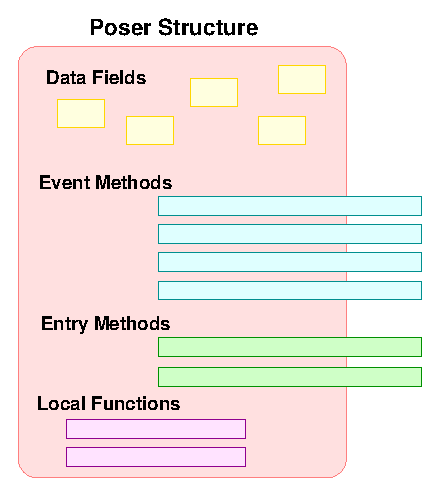
\includegraphics[width=1.5in]{fig/base_struct}
%\end{center}
%\caption{The user's view of a {\it poser}, or simulation object, in \pose{}.}
%\label{fig:base_struct}
%\end{figure}
%
%\section{Delving Deeper into \pose{}}
%
%This section describes some of the internal representations used by
%\pose{}, and how to write more efficient parallel discrete event
%simulations.  The first part deals with how \pose{} simulation objects, or
%{\it posers}, are represented in \pose{}.  It is useful to know a little
%about this internal representation, when deciding what sort of
%sychronization strategy and global state representation to use.  It is
%also essential to know this structure if you want to add new
%strategies and representations.  Even the simulation wrapper class
%(described below) could be subclassed, to modify how the event queue
%gets handled. 
%
%\begin{figure}[h]
%\centering
%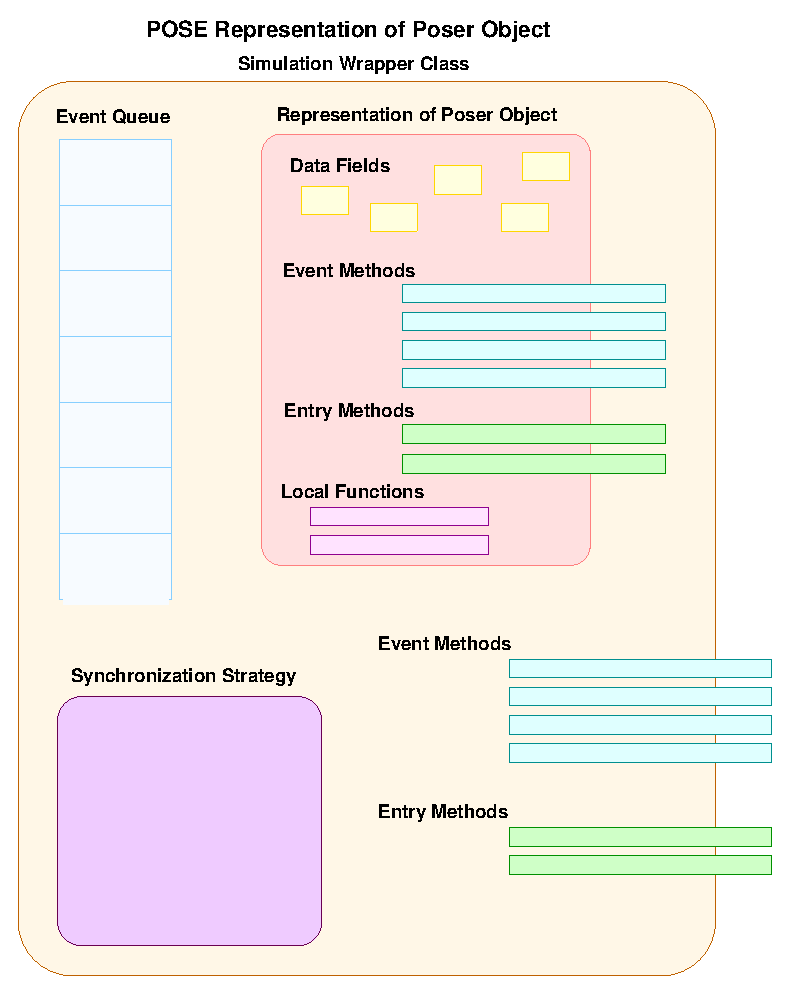
\includegraphics[width=2.5in]{fig/pose_struct}
%\hskip0.5in
%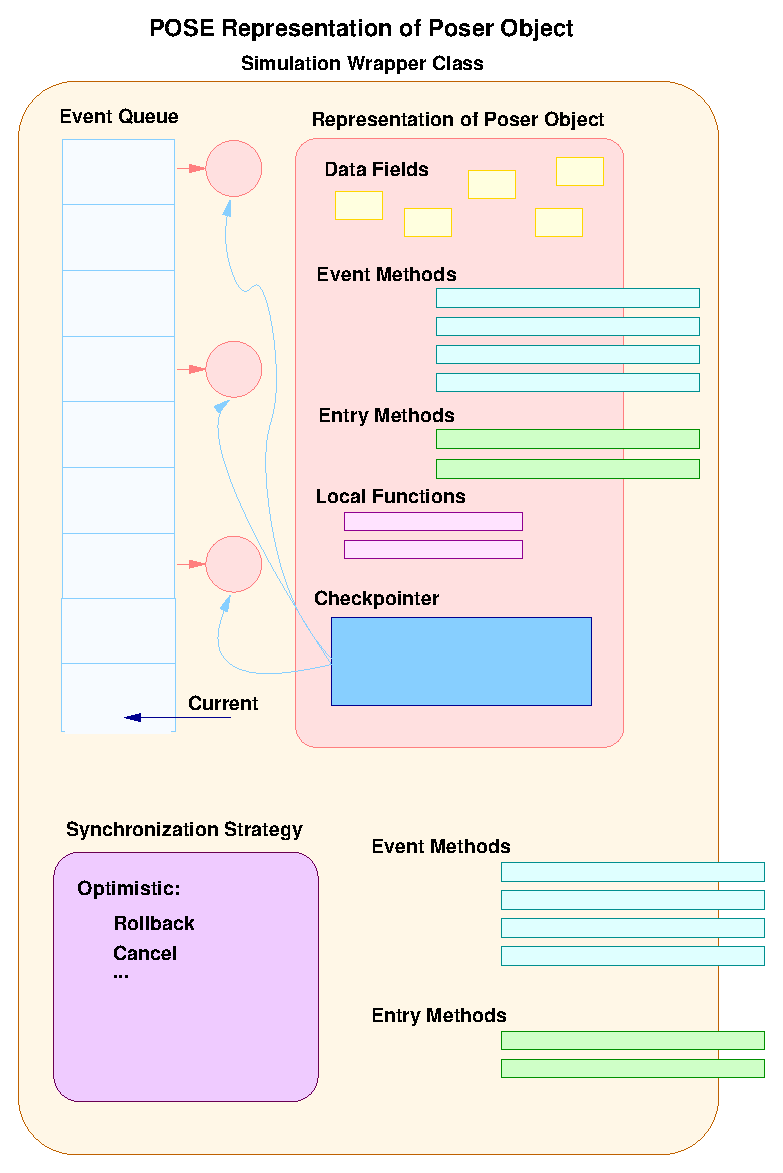
\includegraphics[width=2.5in]{fig/opt_struct}
%\hskip1.7in(a)\hskip2.2in(b)\\
%\caption{(a) Internal representation of a {\it poser}; (b) internal representation of a {\it poser} using optimistic
%synchronization and checkpointing.}
%\label{fig:pose_struct}
%\end{figure}
%
%\subsection{Structure}
%
%The user of \pose{} expresses a simulation object that looks very similar
%to a C++ or Charm++ object.  This poser has data fields that make up a
%part of the simulations global state, and events, which look nearly
%identical to Charm++ entry methods.  Further, it can have ordinary
%Charm++ entry methods, as well as its own internal helper functions.  
%
%\pose{} provides a translator which translates posers into a represention
%that controls access to the object by catching all incoming events to
%the object, placing them in an event queue, and processing them
%according to some strategy.
%
%This internal representation varies based on what synchronization
%strategy and global state representation has been selected.  For
%example, if an optimistic synchronization strategy is used along with a
%checkpointing representation, the internal structure would look like
%that in Fig. ?(b).

%%\subsection{Continuously Changing Simulation Objects with Discrete Behavior Changes}

\end{document}
